\documentclass[11pt, reqno]{amsart}
\usepackage[margin=1in]{geometry}    
\geometry{letterpaper}       
%\geometry{landscape}                % Activate for for rotated page geometry
\usepackage[parfill]{parskip}    % Deactivate to begin paragraphs with an indent rather than an empty line
\usepackage{amsfonts, amscd, amssymb, amsthm, amsmath}
\usepackage{pdfsync}  %leaves makers for tex searching
\usepackage{enumerate}
\usepackage{multicol}
\usepackage[pdftex,bookmarks]{hyperref}

\setlength\parindent{0pt}

%%% Theorems %%%--------------------------------------------------------- 
\theoremstyle{plain}
	\newtheorem{thm}{Theorem}[section]
	\newtheorem{lemma}[thm]{Lemma}
	\newtheorem{prop}[thm]{Proposition}
	\newtheorem{cor}[thm]{Corollary}
\theoremstyle{definition}
	\newtheorem*{defn}{Definition}
	\newtheorem{remark}{Remark}
\theoremstyle{example}
	\newtheorem*{example}{Example}


%%% Environments %%%--------------------------------------------------------- 
\newenvironment{ans}{\color{black}\medskip \paragraph*{\emph{Answer}.}}{\hfill \break  $~\!\!$ \dotfill \medskip }
\newenvironment{sketch}{\medskip \paragraph*{\emph{Proof sketch}.}}{ \medskip }
\newenvironment{summary}{\medskip \paragraph*{\emph{Summary}.}}{  \hfill \break  \rule{1.5cm}{0.4pt} \medskip }
\newcommand\Ans[1]{\color{black}\hfill \emph{Answer:} {#1}}


%%% Pictures %%%--------------------------------------------------------- 
%%% If you need to draw pictures, tikzpicture is one good option. Here are some basic things I always use:
\usepackage{tikz}
\usetikzlibrary{arrows}
\tikzstyle{V}=[draw, fill =black, circle, inner sep=0pt, minimum size=2pt]
\newcommand\TikZ[1]{\begin{matrix}\begin{tikzpicture}#1\end{tikzpicture}\end{matrix}}



%%% Color  %%%---------------------------------------------------------
\usepackage{color}
\newcommand{\blue}[1]{{\color{blue}#1}}
\newcommand{\NOTE}[1]{{\color{blue}#1}}
\newcommand{\MOVED}[1]{{\color{gray}#1}}


%%% Alphabets %%%---------------------------------------------------------
%%% Some shortcuts for my commonly used special alphabets and characters.
\def\cA{\mathcal{A}}\def\cB{\mathcal{B}}\def\cC{\mathcal{C}}\def\cD{\mathcal{D}}\def\cE{\mathcal{E}}\def\cF{\mathcal{F}}\def\cG{\mathcal{G}}\def\cH{\mathcal{H}}\def\cI{\mathcal{I}}\def\cJ{\mathcal{J}}\def\cK{\mathcal{K}}\def\cL{\mathcal{L}}\def\cM{\mathcal{M}}\def\cN{\mathcal{N}}\def\cO{\mathcal{O}}\def\cP{\mathcal{P}}\def\cQ{\mathcal{Q}}\def\cR{\mathcal{R}}\def\cS{\mathcal{S}}\def\cT{\mathcal{T}}\def\cU{\mathcal{U}}\def\cV{\mathcal{V}}\def\cW{\mathcal{W}}\def\cX{\mathcal{X}}\def\cY{\mathcal{Y}}\def\cZ{\mathcal{Z}}

\def\AA{\mathbb{A}} \def\BB{\mathbb{B}} \def\CC{\mathbb{C}} \def\DD{\mathbb{D}} \def\EE{\mathbb{E}} \def\FF{\mathbb{F}} \def\GG{\mathbb{G}} \def\HH{\mathbb{H}} \def\II{\mathbb{I}} \def\JJ{\mathbb{J}} \def\KK{\mathbb{K}} \def\LL{\mathbb{L}} \def\MM{\mathbb{M}} \def\NN{\mathbb{N}} \def\OO{\mathbb{O}} \def\PP{\mathbb{P}} \def\QQ{\mathbb{Q}} \def\RR{\mathbb{R}} \def\SS{\mathbb{S}} \def\TT{\mathbb{T}} \def\UU{\mathbb{U}} \def\VV{\mathbb{V}} \def\WW{\mathbb{W}} \def\XX{\mathbb{X}} \def\YY{\mathbb{Y}} \def\ZZ{\mathbb{Z}}  

\def\fa{\mathfrak{a}} \def\fb{\mathfrak{b}} \def\fc{\mathfrak{c}} \def\fd{\mathfrak{d}} \def\fe{\mathfrak{e}} \def\ff{\mathfrak{f}} \def\fg{\mathfrak{g}} \def\fh{\mathfrak{h}} \def\fj{\mathfrak{j}} \def\fk{\mathfrak{k}} \def\fl{\mathfrak{l}} \def\fm{\mathfrak{m}} \def\fn{\mathfrak{n}} \def\fo{\mathfrak{o}} \def\fp{\mathfrak{p}} \def\fq{\mathfrak{q}} \def\fr{\mathfrak{r}} \def\fs{\mathfrak{s}} \def\ft{\mathfrak{t}} \def\fu{\mathfrak{u}} \def\fv{\mathfrak{v}} \def\fw{\mathfrak{w}} \def\fx{\mathfrak{x}} \def\fy{\mathfrak{y}} \def\fz{\mathfrak{z}}
\def\fgl{\mathfrak{gl}}  \def\fsl{\mathfrak{sl}}  \def\fso{\mathfrak{so}}  \def\fsp{\mathfrak{sp}}  
\def\GL{\mathrm{GL}} \def\SL{\mathrm{SL}}  \def\SP{\mathrm{SL}}

\def\<{\langle} \def\>{\rangle}
\usepackage{mathabx}
\def\acts{\lefttorightarrow}
\def\ad{\mathrm{ad}} 
\def\Aut{\mathrm{Aut}}
\def\Ann{\mathrm{Ann}}
\def\dim{\mathrm{dim}} 
\def\End{\mathrm{End}} 
\def\ev{\mathrm{ev}} 
\def\Fr{\mathcal{F}\mathrm{r}}
\def\half{\hbox{$\frac12$}}
\def\Hom{\mathrm{Hom}} 
\def\id{\mathrm{id}} 
\def\sgn{\mathrm{sgn}}  
\def\supp{\mathrm{supp}}  
\def\Tor{\mathrm{Tor}}
\def\tr{\mathrm{tr}} 
\def\vep{\varepsilon}
\def\f{\varphi}


\def\Obj{\mathrm{Obj}}
\def\normeq{\unlhd}
\def\Set{{\cS\mathrm{et}}}
\def\Fin{{\cF\mathrm{inSet}}}
\def\Set{{\cS\mathrm{et}}}
\def\Grp{{\cG\mathrm{rp}}}
\def\Ab{{\cA\mathrm{b}}}
\def\Mod{{\cM\mathrm{od}}}
\def\ab{\mathrm{ab}}
\def\lcm{\mathrm{lcm}}
\def\ZZn{\ZZ/n\ZZ}


%%%%%%%%%%%%%%%%%%%%%%%%%%%%%% 
%%%%%%%%%%%%%%%%%%%%%%%%%%%%%%

\def\HW{5}
\def\DUE{10/18/2020}

\title[Homework \HW]{Homework \HW \\
Math A4900/44900\\
\small Due: \DUE}
\author{}

\begin{document}
%\maketitle %%% COMMENT THIS LINE OUT (add a % to the beginning of the line) and UNCOMMENT the following (delete the % symbols) to give yourself a good assignment header:
\begin{flushright}
Chris Hayduk\\
Math A4900\\
Research Paper Summaries\\
\DUE
\end{flushright}

\section{Introduction}
\indent
The main paper in this research summary, \textit{Lambek vs. Lambek: functorial vector space semantics and string diagrams for Lambek calculus}, was published in the Annals of Pure and Applied Logic in June 2013 and was written by Bob Coecke, Edward Grefenstette, and Mehrnoosh Sadrazdeh \cite{lambekvlambek}. Bob Coeke is a currently theoretical physicist at the University of Oxford. He received his doctorate degree from Vrije Universiteit Brussel in 1996 and went on to perform postdoctoral work at Imperial College, London and McGill University in Montreal. During the time that this paper was written, Bob Coeke was a professor of Quantum Foundations, Logic, and structures at Oxford. He stills holds this position today. His research interests include category theory, logic, and diagrammatic reasoning \cite{coecke}.
\par
Edward Grefenstette is currently a research scientist at Facebook AI and an honorary Associate Professor at University College London (UCL). He received his PhD in Computer Science from the University of Oxford in 2013. Following his PhD, he worked as a postdoctoral research assistant in the Computer Science department at Oxford. Grefenstette then moved to DeepMind in London before finally joining Facebook AI. His research primarily focuses on applying category theory and deep learning to natural language processing problems \cite{grefenstette}.
\par
Mehrnoosh Sadrazdeh is currently an Associate Professor in the Programming Principles, Logic, and Verification Group at University College London. From 2008 to 2013, she was a Postdoctoral Fellow and a Research Fellow in the Computer Science Department of the University of Oxford. Following this, she became a lecturer in the School Electronic Engineering and Computer Science at Queen Mary University of London from 2013 to 2019. Her research interests include natural language processing (NLP) and high-level logical models for computer systems \cite{sadrzadeh}.
\par
Their paper, \textit{Lambek vs. Lambek: functorial vector space semantics and string diagrams for Lambek calculus}, is an application of categorial grammar, which is a view of a natural language syntax which states that the components of a sentence behave as functions \cite{categorialgrammar}. The authors of the paper make use of Lambek's pregroup grammar in order to model the type-logic of the sentences. Lambek's pregroup grammar is a simplification of Lambek calculus, which has been used in various contexts in mathematical and computational linguistics. This pregroup grammar provides a computational procedure when can be used, in conjunction with the definitions of the words, to construct a meaning for any given sentence. More popular approaches in natural language processing currently purely use word meanings based on context in order to construct the meanings of sentences. These models are known as empirical models of semantics, and they have been very successful in quite a few applications, such as thesaurus extraction. In this paper, the authors create the distributional compositional categorical (DisCoCat) model of meaning, which combines the logical framework of Lambek's pregroup grammar with the contextual word definitions of empirical models in order to improve performance in specific natural language processing tasks, such as word-sense disambiguation \cite{lambekvlambek}.
\newpage
\section{Summary}

In this paper, the authors construct a form of categorial grammar using Lambek's pregroup grammar. They begin with a description of Lambek calculus. It consists of a non-commutative binary operation on partially ordered sets. The authors then go on to define a residuated monoid as follows,

\par
\textbf{Definition 2.1} \cite{lambekvlambek} A residuated monoid is a partially ordered set $(L, \leq)$ equipped with a monoid structure $(L, \cdot, 1)$ that preserves the partial order, that is for all $a, b, c \in L$, we have,
\begin{align*}
\text{If} \; a \leq b \; \text{then} \; a \cdot c \leq b \cdot c \; \text{and} \; c \cdot a \leq c \cdot b
\end{align*}

Note that a monoid has a single associative binary operation and an identity element \cite{monoid}. A partially ordered residuated monoid is called a Lambek monoid in the context of this paper \cite{lambekvlambek}. In addition, we have the following definitions for a natural language and a Lambek grammar,
\par
\textbf{Definition 2.2} \cite{lambekvlambek} For $\Sigma$ the set of words of a natural language and $\mathcal{B}$ a set of basic grammatical types, a Lambek type-dictionary is binary relation $D$ defined as
\begin{align*}
D \subset \Sigma \times T(\mathcal{B})
\end{align*}

where $T(B)$ is the free Lambek monoid generated over $\mathcal{B}$

\par
\textbf{Definition 2.3} \cite{lambekvlambek} A Lambek grammar $G$ is a pair $\langle D, S \rangle$, where $D$ is a Lambek type-dictionary and $S \subset \mathcal{B}$ is a set of designated types, containing types such as that of a declarative sentence $s$ and a question $q$.

\par
Thus, as we can see, a Lambek-type dictionary assigns each word in the language a structure from the free Lambek monoid generated over $\mathcal{B}$. The Lambek grammar then assigns another type to each ordered pair in $D$.

\par
Lambek later developed a simplification for his Lambek grammar in which he used a pregroup structure. The definition is as follows,

\par
\textbf{Definition 2.5} \cite{lambekvlambek} A Lambek pregroup is a partially ordered unital monoid where each element has a left and a right adjoint $(P, \leq, \cdot, 1, (-)^{\ell}, (-)^r)$. That is, for every $p \in P$, there is a $p^r$ and a $p^{\ell}$ in $P$, which satisfy the following four inequalities:
\begin{align*}
p \cdot p^r \leq &1 \leq p^r \cdot p\\
p^{\ell} \cdot p \leq &1 \leq p \cdot p^{\ell}
\end{align*}

\par
The authors gave the following example for a Lambke pregroup grammar,\\
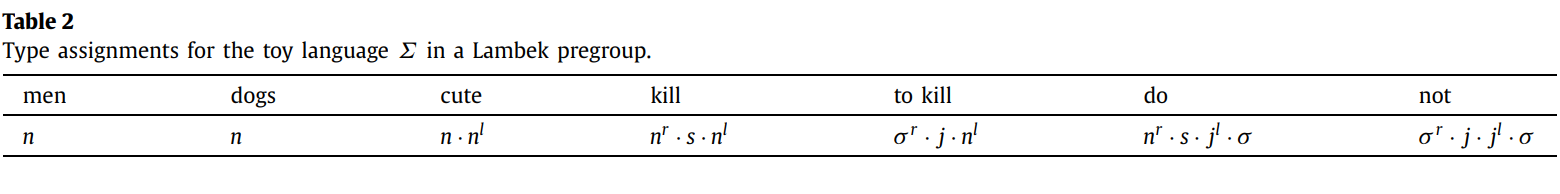
\includegraphics[scale=0.55]{lambek_pregroup}

\par
Each word in the language is assigned a specific grammatical role, represented by some combination of elements in the Lambek pregroup. The meaning of a sentence can then be determined by composing these elements together as functions in the order in which they appear in the sentence.

\par
The authors then went on to describe distributional models of meaning, which model words based on their meaning in context. The language is depicted as a vector space, and usually several important words are selected in order to form a basis for the vector space in which each word vector lives. The angle between word vectors is used as a proxy for the closeness in meaning between those two words, as the angle is smaller for words that appear in similar context. For example, the word vectors ``cat'' and ``dog'' would have a smaller angle than the word vectors ``cat'' and ``democracy'' because ``cat'' and ``dog'' appear in very similar contexts. The authors give the following image on p. 7 of the paper in order to graphically explain this concept,\\

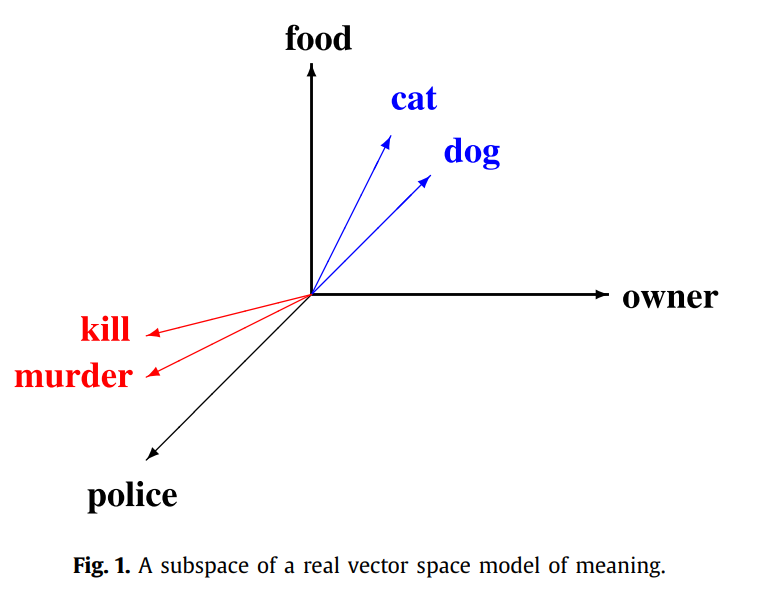
\includegraphics[scale=0.7]{vector_space}

\par
These models ignore the grammatical structure of the language, unlike the Lambek pregroup grammar discussed previously. There is also an issue with sentences of differing lengths. For example, a distributional model of meaning cannot compare the sentences ``I walk the dog'' and ``I walk'' because they live in different spaces. The authors discuss that a way to resolve these issues is to combine the pregroup grammar with a distributional model. This allows the model to produce vectors for the meanings of sentences, taking into account both the grammatical structure of the sentence and the word vectors contained within it. The paper proposes the following definition for their DisCoCat model,

\par
\textbf{Definition 4.1} \cite{lambekvlambek} The distributional compositional categorical (DisCoCat) model of meaning is a category $FVect \times Preg$, equipped with a tensor product given by pointwise tensor of $Preg$ and $FVect$, that is $(V, p) \otimes (W, q) = (V \otimes W, p \cdot q)$, whose unit is $(\RR, 1)$.

\par
where $FVect$ is the finite dimensional vector space of word meanings and $Preg$ is he pregroup grammar. Both the pregroup grammar and the finite dimensional vector space form compact closed categories \cite{lambekvlambek}.

\section{Reflection}

\par
This paper adds onto the current literature in categorial grammar by extending the DisCoCat model from pregroups to Lambek monoids \cite{lambekvlambek}. This allows the model to more closely relate to semantic models of language \cite{lambekvlambek}. In addition, the method of constructing the DisCoCat model can be extended to other domains, and in particular has been used in Topological Quantum Field Theory. The authors describe their work here as a ``grammatical quantum field theory for Lambek monoids'' \cite{lambekvlambek}. I personally had a strong interest in this paper due to my interest in language learning and linguistics. I find the diverse structures of natural language and the rules that govern its grammar to be very interesting, and I believe mathematical linguistics is important in analyzing the general rules that are common among natural language grammars. Moreover, I think Natural Language Processing is one of the most exciting fields in Machine Learning, so seeing the connections between algebra and category theory with more traditional NLP approaches was great.

\par
The authors of this paper made use of a significant number of definitions and images in order to explain the background of this topic. I found this to be very helpful in building up some understanding for and intuition of the objects that were being discussed. Unfortunately there was still a large amount of background knowledge that I was lacking which made parts of the paper difficult to parse. However, overall, I think the writing style of the paper and clarity of exposition made this paper easier to digest than many other papers that I have seen.

\appendix
\section{Follow-up Papers}

\par
In the paper, \textit{A generalised quantifier theory of natural language in categorical compositional distributional semantics with bialgebras}, the authors expand on the work in categorical compositional distributional semantics which was discussed in \textit{Lambek vs. Lambek}. The authors in this paper formalize and generalize this approach to natural language modeling \cite{quantifier}. The authors of this paper include Mehrnoosh Sadrzadeh, who was an author on the \textit{Lambek vs. Lambek} paper, as well as Jules Hedges. Hedges received his PhD from the University of Oxford and, at the time of the paper's publication, was a postdoctoral researcher at the Max Planck Institute for Mathematics in the Sciences \cite{hedges}.

\par
In the paper, \textit{Generalized Relations in Linguistics and Cognition}, the authors expand the categorical compositional models of natural language which were discussed in \textit{Lambek vs. Lambek} to conceptual space models of cognition \cite{relations}. This builds on what was stated in \textit{Lambek vs. Lambek}, that the categorical compositional model described a generalized approach which could be applied to other domains \cite{lambekvlambek}. The authors of this paper included Bob Coecke, who was included on the \textit{Lambek vs. Lambek} paper. In addition, the authors included Fabrizio Genovese, who was a PhD student at the University of Oxford at the time of the paper's publication \cite{genovese}. We also have Martha Lewis, a research assistant at Oxfrod with research interests in modeling how humans represent and use concepts in their minds \cite{lewis}. Lastly, Dan Marsden is a research assistant at Oxford whose research interests include category theoretic techniques to model systems in areas such as quantum computation and natural language semantics \cite{marsden}.

\begin{thebibliography}{9}
\bibitem{lambekvlambek} 
Coecke, Bob;  Grefenstette, Edward; Sadrzadeh, Mehrnoosh. \textit{Lambek vs. Lambek: functorial vector space semantics and string diagrams for Lambek calculus}. Ann. Pure Appl. Logic  164  (2013),  no. 11, 1079--1100.

\bibitem{quantifier} 
Hedges, Jules; Sadrzadeh, Mehrnoosh. \textit{A generalised quantifier theory of natural language in categorical compositional distributional semantics with bialgebras}. Math. Structures Comput. Sci.  29  (2019),  no. 6, 783--809.

\bibitem{relations} 
Coecke, Bob; Genovese, Fabrizio; Lewis, Martha; Marsden, Dan. \textit{Generalized Relations in Linguistics and Cognition}. Logic, Language, Information, and Computation (2017), pp. 256--270.

\bibitem{coecke}
“Bob Coecke.” Wikipedia, Wikimedia Foundation, 18 Oct. 2020, \texttt{en.wikipedia.org/wiki/Bob\_Coecke}.

\bibitem{grefenstette}
“Edward Grefenstette.” 18 Oct. 2020, \texttt{https://www.egrefen.com/}

\bibitem{sadrzadeh}
“Mehrnoosh Sadrzadeh.” 18 Oct. 2020, \texttt{https://msadrzadeh.com/}

\bibitem{categorialgrammar}
“Categorial Grammar.” Wikipedia, Wikimedia Foundation, 30 Aug. 2020, \\\texttt{en.wikipedia.org/wiki/Categorial\_grammar}. 

\bibitem{monoid}
“Monoid.” Wikipedia, Wikimedia Foundation, 18 Oct. 2020, \texttt{en.wikipedia.org/wiki/Monoid}. 

\bibitem{hedges}
“CV.” \textit{Jules Hedges}, 21 Aug. 2020, \texttt{julesh.com/cv/}. 

\bibitem{genovese}
“Fabrizio Romano Genovese.” 19 Oct. 2020, \texttt{www.cs.ox.ac.uk/people/fabrizio.genovese/}. 

\bibitem{lewis}
“Martha Lewis.” 19 Oct. 2020, \texttt{https://www.cs.ox.ac.uk/people/martha.lewis/}. 

\bibitem{marsden}
“Dan Marsden.” 19 Oct. 2020, \texttt{https://www.cs.ox.ac.uk/people/dan.marsden/}. 
\end{thebibliography}



\end{document}